\chapter{Finite State Machines}
\graphicspath{ {./chapter07/FigWork} }

%%%%%%%%%%%%%%%%%%%%%%%%%%%%%%%%%%%%%%%%%%%%%%%%%%%%
%% Here are the helpful stuff
%%%%%%%%%%%%%%%%%%%%%%%%%%%%%%%%%%%%%%%%%%%%%%%%%%%%
\section{Helpful Stuff}

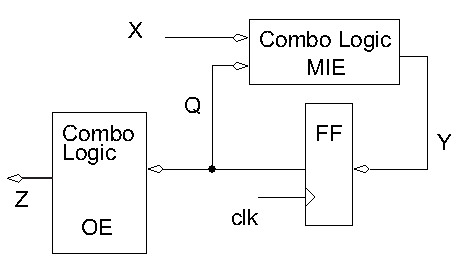
\includegraphics{../Fig/GenFSM}


%%%%%%%%%%%%%%%%%%%%%%%%%%%%%%%%%%%%%%%%%%%%%%%%%%%%
%% Here are terms that the students define
%%%%%%%%%%%%%%%%%%%%%%%%%%%%%%%%%%%%%%%%%%%%%%%%%%%%



%%%%%%%%%%%%%%%%%%%%%%%%%%%%%%%%%%%%%%%%%%%%%%%%%%%%
%% Here are the problems
%%%%%%%%%%%%%%%%%%%%%%%%%%%%%%%%%%%%%%%%%%%%%%%%%%%%
\section{Problems}

\begin{description}
\item[Convert the state diagram into a state table.]
The input variable is $X$.

\begin{tabular}{ll}
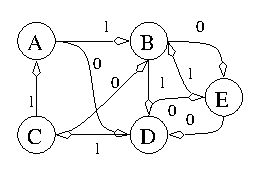
\includegraphics{StateDiagram} &
\begin{tabular}{c||c|c}
CURRENT STATE	& X=0	& X=1	\\ \hline
A		& 	& 	\\ \hline
B		& 	& 	\\ \hline
C		& 	& 	\\ \hline
D		& 	& 	\\ \hline
E		&	& 	\\ 
\end{tabular} \\
	& entries should be next state
\end{tabular}
\pagebreak

\item[Convert the state table into a transistion kmap.]  Use the 
state assignment provided.

\begin{tabular}{ll}
\begin{tabular}{c||c}
State & $Q_2 Q_1 Q_0$	\\ \hline
A	& 010		\\ \hline
B	& 101		\\ \hline
C	& 100		\\ \hline
D	& 001		\\ \hline
E	& 011		\\ 
\end{tabular} 
&
\begin{tabular}{c|c|c|c|c}
$Q_2 Q_1 \bs Q_0 X$	& 00	& 01	& 11	& 10	\\ \hline
00 			& 	& 	&	&	\\ \hline
01			& 	& 	&	&	\\ \hline
11			& 	& 	&	&	\\ \hline
10			&	& 	&	&	\\ 
\end{tabular} \\
	& entries should be $Q_2^+ Q_1^+ Q_0^+$
\end{tabular}

\item[Determine the memory input equations.]  Use the transition
kmap given in the previous problem.

$$\begin{array}{c}
\begin{array} {c||c|c|c|c}
        Q_2 Q_1 \bs Q_0 X	&  00 &  01 &  11 &  10 \\ \hline
        00				& & & &  \\ \hline
        01				& & & &  \\ \hline
        11				& & & &  \\ \hline
        10				& & & &  \\
\end{array} \\

\begin{array} {c||c|c|c|c}
        Q_2 Q_1 \bs Q_0 X	&  00 &  01 &  11 &  10 \\ \hline
        00				& & & &  \\ \hline
        01				& & & &  \\ \hline
        11				& & & &  \\ \hline
        10				& & & &  \\
\end{array} \\

\begin{array} {c||c|c|c|c}
        Q_2 Q_1 \bs Q_0 X	&  00 &  01 &  11 &  10 \\ \hline
        00				& & & &  \\ \hline
        01				& & & &  \\ \hline
        11				& & & &  \\ \hline
        10				& & & &  \\
\end{array} 

\end{array} $$
\pagebreak


\item[Write the MIEs]  Assume a 1's hot encoding of the states.

\begin{tabular}{ll}
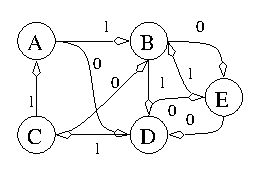
\includegraphics{StateDiagram}  &
	\begin{tabular}{l}
	$D_A$= \\
	$D_B$= \\
	$D_C$= \\
	$D_D$= \\
	$D_E$= \\
	$Z$= \\
	\end{tabular}
\end{tabular}
\vspace{1.0in}

\item[Write the MIEs]  Use the state Assume a 1's hot encoding of the states.

\begin{tabular}{ll}
\begin{tabular}{c||c|c}
Q	& X=0	& X=1 \\ \hline
A	& C	& C	\\ \hline
B	& D	& A	\\ \hline
C	& D	& E	\\ \hline
D	& A	& E	\\ \hline
E	& C	& B	\\ 
\end{tabular}
&
	\begin{tabular}{l}
	$D_A$= \\
	$D_B$= \\
	$D_C$= \\
	$D_D$= \\
	$D_E$= \\
	$Z$= \\
	\end{tabular}
\end{tabular}

\pagebreak

\item[Given the state table and state assignment determine the MIEs.]

\begin{tabular}{ll}
\begin{tabular}{c||c|c|c|c}
State & ND=00 & ND = 01 & ND=11 & ND=10 \\ \hline
0     & 0	& 10	  & x	  & 5 	  \\ \hline
5     & 5	& 15	  & x	  & 10 	  \\ \hline
10    & 10	& 20	  & x	  & 15 	  \\ \hline
15    & 15	& 25	  & x	  & 20 	  \\ \hline
20    & 20	& 30	  & x	  & 25 	  \\ \hline
25    & 25	& 35	  & x	  & 30 	  \\ \hline
30    & 30	& 35	  & x	  & 35 	  \\ \hline
35    & 0	& 0	  & x	  & 0 	  \\ 
\end{tabular}
&

$\begin{array}{c|c|c|c}
\text{ state} & Q_2 & Q_1 & Q_0 \\ \hline
0  & 0 & 0 & 0 \\ \hline
5  & 0 & 0 & 1 \\ \hline
10 & 0 & 1 & 0 \\ \hline
15 & 0 & 1 & 1 \\ \hline
20 & 1 & 0 & 0 \\ \hline
25 & 1 & 0 & 1 \\ \hline
30 & 1 & 1 & 0 \\ \hline
35 & 1 & 1 & 1 \\ 
\end{array}$ \\
\end{tabular}

$$\begin{array}{cc}
\begin{array} {c||c|c|c|c}
        Q_1 Q_0 \bs ND  &  00 &  01 &  11 &  10 \\ \hline
        00              & & & &  \\ \hline
        01              & & & &  \\ \hline
        11              & & & &  \\ \hline
        10              & & & &  \\
\end{array}
&
\begin{array} {c||c|c|c|c}
        Q_1 Q_0 \bs ND  &  00 &  01 &  11 &  10 \\ \hline
        00              &  &  &  &  \\ \hline
        01              &  &  &  &  \\ \hline
        11              &  &  &  &  \\ \hline
        10              &  &  &  &  \\
\end{array} \\
Q_2=0 & Q_2=1 \\
\multicolumn{2}{c}{\text{ Entries\ are\ } Q_2^+ Q_1^+ Q_0^+}
\end{array} $$

{\tiny
$$\begin{array}{cc}
\begin{array} {c||c|c|c|c}
	Q_1 Q_0 \bs ND	& 00 & 01 & 11 & 10 \\ \hline
        00        	&    &   &   &    \\ \hline
        01        	&    &   &   &    \\ \hline
        11        	&    &   &   &   \\ \hline
        10        	&    &   &   &    \\
\end{array}
&
\begin{array} {c||c|c|c|c}
	Q_1 Q_0 \bs ND	& 00 & 01 & 11 & 10 \\ \hline
        00        	&   &   &   &   \\ \hline
        01        	&   &   &   &   \\ \hline
        11        	&   &   &   &   \\ \hline
        10        	&   &   &   &   \\
\end{array} \\
Q_2=0 & Q_2=1 \\
\multicolumn{2}{c}{\text{ Entries\ are\ } Q_2^+=D_2}
\end{array} $$

$$\begin{array}{cc}
\begin{array} {c||c|c|c|c}
	Q_1 Q_0 \bs ND	& 00 & 01 & 11 & 10 \\ \hline
        00        	&    &   &   &    \\ \hline
        01        	&    &   &   &    \\ \hline
        11        	&    &   &   &   \\ \hline
        10        	&    &   &   &    \\
\end{array}
&
\begin{array} {c||c|c|c|c}
	Q_1 Q_0 \bs ND	& 00 & 01 & 11 & 10 \\ \hline
        00        	&   &   &   &   \\ \hline
        01        	&   &   &   &   \\ \hline
        11        	&   &   &   &   \\ \hline
        10        	&   &   &   &   \\
\end{array} \\
Q_2=0 & Q_2=1 \\
\multicolumn{2}{c}{\text{ Entries\ are\ } Q_1+=D_1}
\end{array} $$


$$\begin{array}{cc}
\begin{array} {c||c|c|c|c}
	Q_1 Q_0 \bs ND	& 00 & 01 & 11 & 10 \\ \hline
        00        	&    &   &   &    \\ \hline
        01        	&    &   &   &    \\ \hline
        11        	&    &   &   &   \\ \hline
        10        	&    &   &   &    \\
\end{array}
&
\begin{array} {c||c|c|c|c}
	Q_1 Q_0 \bs ND	& 00 & 01 & 11 & 10 \\ \hline
        00        	&   &   &   &   \\ \hline
        01        	&   &   &   &   \\ \hline
        11        	&   &   &   &   \\ \hline
        10        	&   &   &   &   \\
\end{array} \\
Q_2=0 & Q_2=1 \\
\multicolumn{2}{c}{\text{ Entries\ are\ } Q_0+=D_0}
\end{array} $$
}


\item[Parity Checker]
When data is transmitted, there is a chance that noise will corrupt some portion of the data.  
To detect errors, a single parity bit can be added to each data item to detect single bit errors.  
The value of the parity bit is determined by the number of 1's in the data packet the parity bit
is being added to.  In an even-parity scheme, the parity bit's value, 0 or 1, is set so that the
number of 1's in the data packet plus the parity bit is an even number.  For example if 
the data packet 1101 0011 has a total of 5 1's.  The even-parity bit would be 1 and 
you would transmit 1101 0011 1, the last 1 being the parity bit.  The parity bit is 
then re-computed by the receive and checked against the transmitted bit.  Clearly,
the transmitter and receiver must agree on the even or odd before the parity bit
is useful.

The following timing diagram and circuit shows a parity checking circuit.  The serial
data input is x and the parity bit is z.  Complete the timing diagram using the circuit
diagram to plug in values at the given time and computing the signal values out of
the gates and the SR flip flop.  you should assume that the SR flip flop is initially
reset (Q = 0).  Does this circuit realize a even or odd parity circuit? 



\begin{figure}[ht]
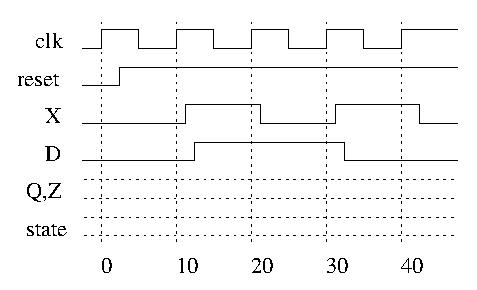
\includegraphics[width=0.6\paperwidth]{ParityTime}
\vspace{0.4cm}
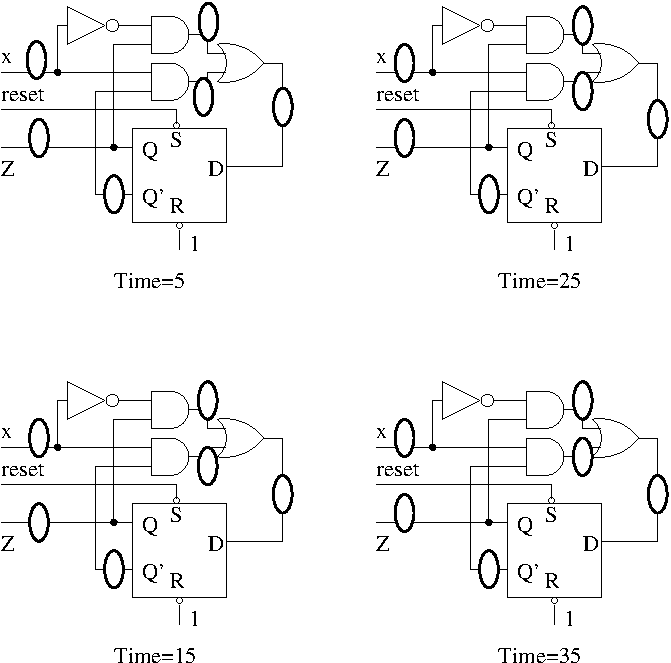
\includegraphics[width=0.5\paperwidth]{ParityAct}
\end{figure}







\end{description}
